% !TEX root = ../../thesis.tex

\cleartoleftpage
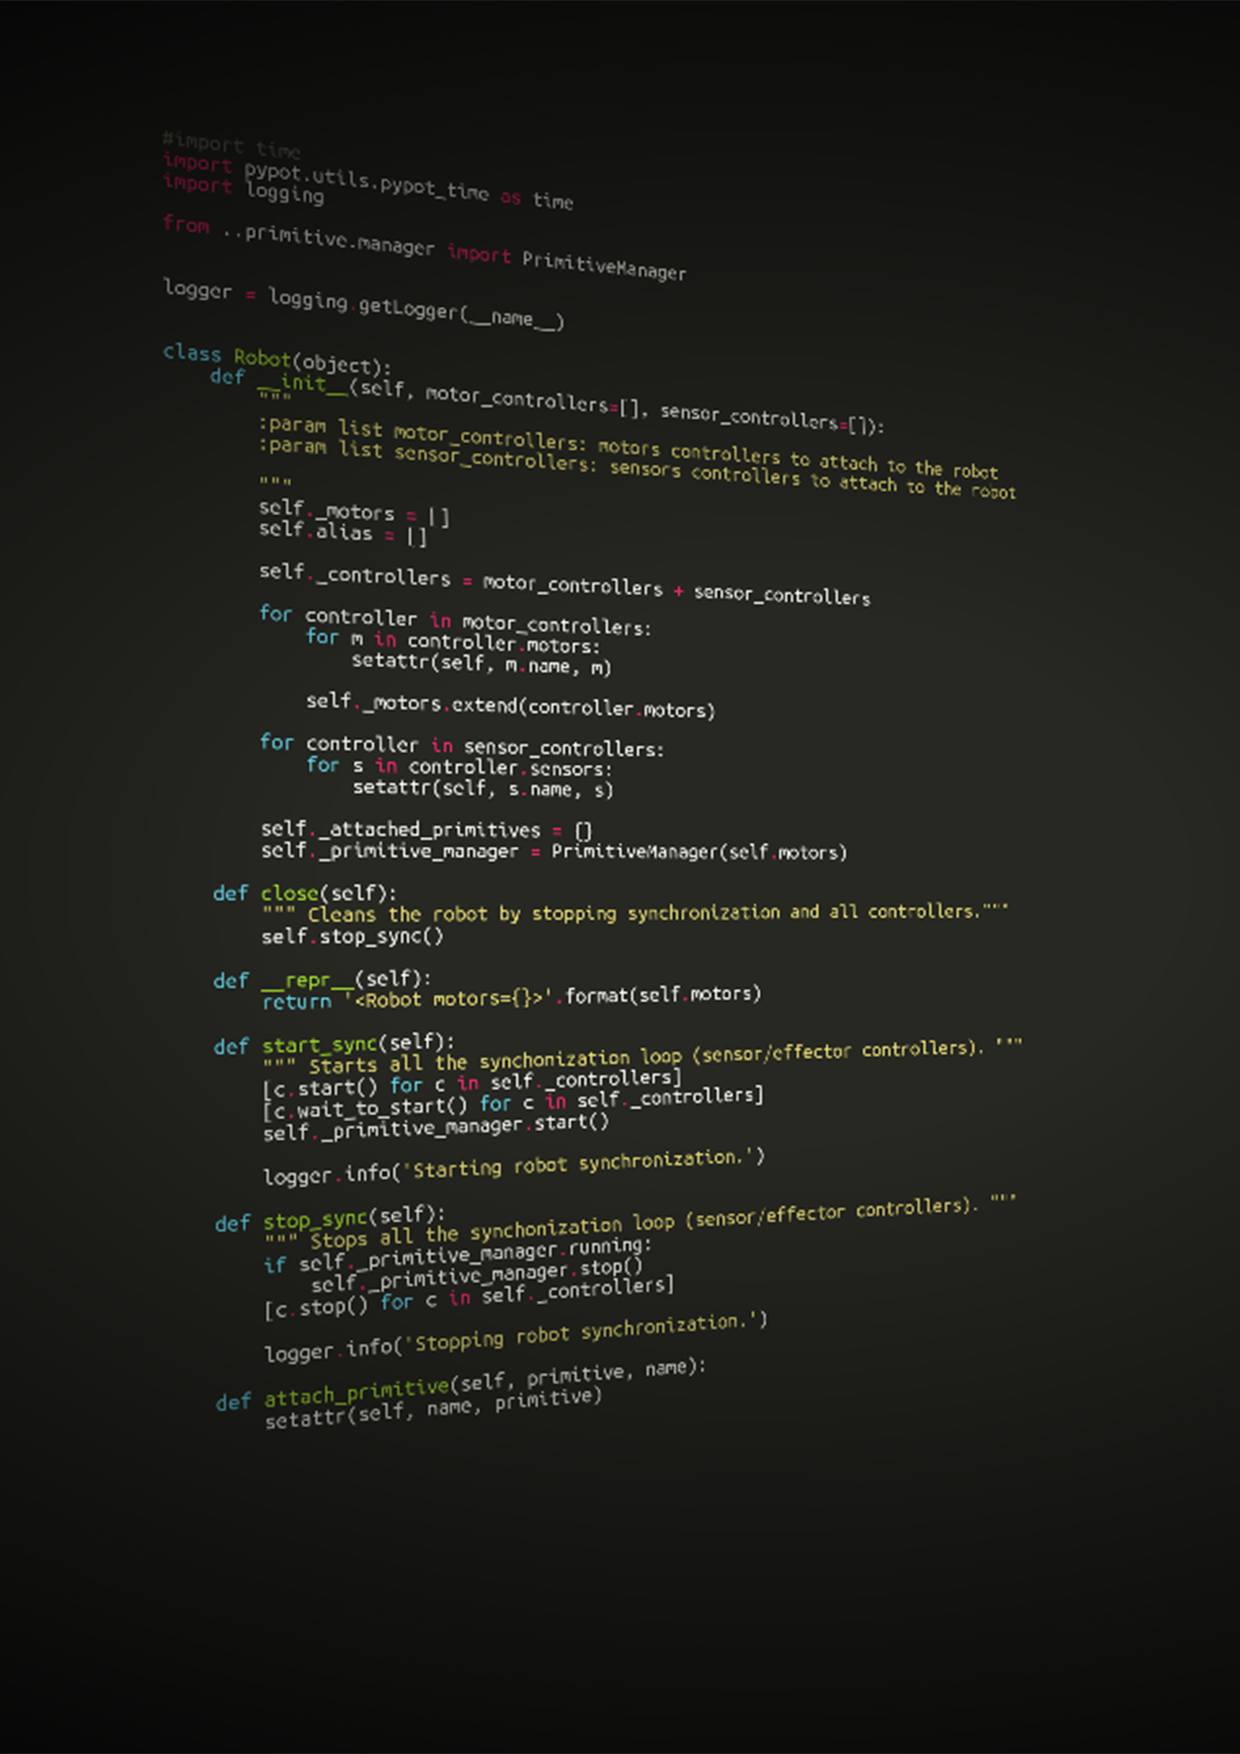
\includepdf{../media/chapter_illustration/pypot}
\chapter{Pypot: An open source modular python library for robot control} % (fold)

\section{Introduction} % (fold)

Poppy was designed to be a research platform for freely exploring morphological variations. Although Poppy meets "hardware" needs, control of the platform is also crucial. Whereas more conventional robots have a fixed mechanical and sensorimotor morphology, having a platform that can be fully modified changes the low-level control architecture issues.
We decided to develop a new robotic control library. Called pypot (see \figurename~\ref{fig:pypot_logo}), this library mostly developed by Pierre Rouanet, is adapted to the challenges of morphological exploration and experimentation. Moreover, development begun early in the design of Poppy, and shares the same guidelines and objectives i.e. being robust, modular, versatile and easy to use.


\begin{NFfigure}
    \centering
        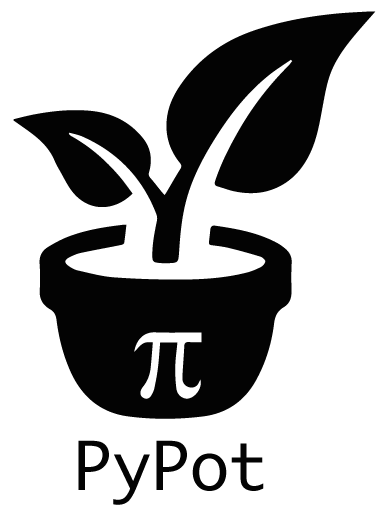
\includegraphics[height=5cm]{PyPot_logo_black_transparentbg.png}
    \caption{The logo of the pypot library.}
    \label{fig:pypot_logo}
\end{NFfigure}

To reach these goals, pypot is a library written in Python and developed to make it easy and fast to control custom and modular robots. In particular, pypot has been designed with a simple and easy to use API, a fully modular and customizable architecture, and key-features adapted to robot experimentation issues.

It also shares the open collaboration philosophy and is therefore distributed under an open source GPLv3 license. All sources are available on the associated GitHub repository: \url{https://github.com/poppy-project/pypot}.

Even if pypot has been developed within the context of the Poppy project, in the following sections, most of the code examples will involve an ergo-robot (see \figurename~\ref{fig:ergo-robot}) rather than Poppy to emphasize that pypot is a control library for any modular robot.


\begin{figure}[tb]
\centering
    \subfloat[][]{\label{fig:cpu-load}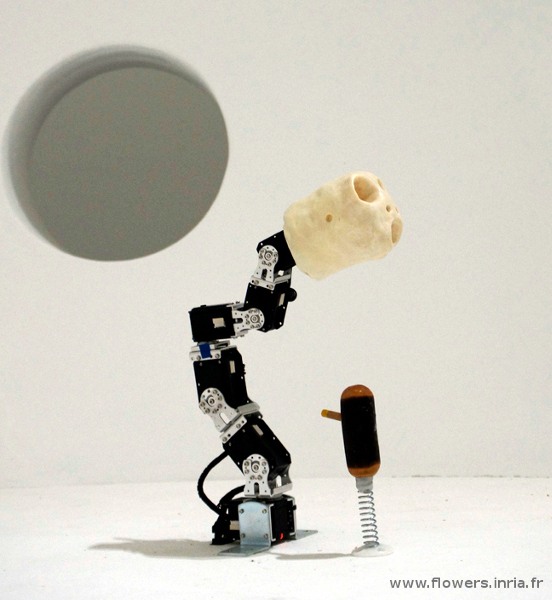
\includegraphics[height=5cm]{ergo-robot-stem.jpg}}
    \hfil
    \subfloat[][]{\label{fig:pypy-opti}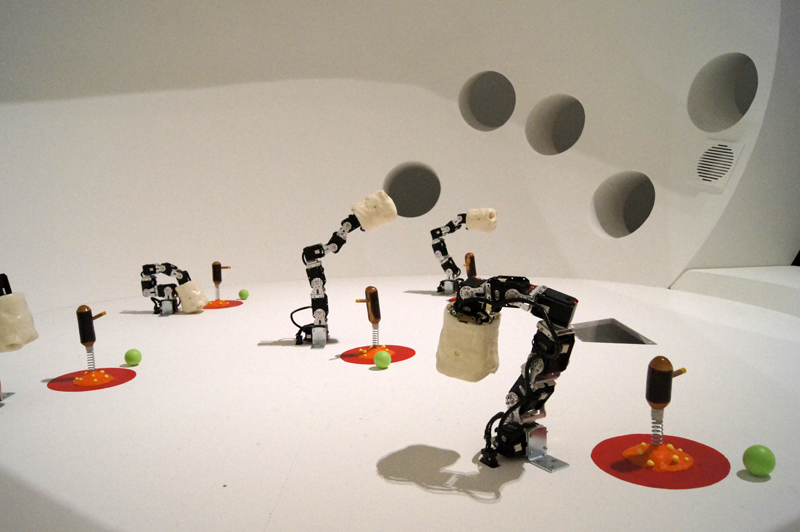
\includegraphics[height=5cm]{ergo-robot.jpg}}
    \caption{Ergo-robot are a 6 DoF serial robots with a stem shape those were developed in the Flowers Lab. In particular, they were involved for the Fondation Cartier exhibition (see chapter~\ref{cha:art})}
    \label{fig:ergo-robot}
\end{figure}


\section{Control of custom robots made simple with pypot} % (fold)

One main preoccupation during the development of pypot was the achievement of a very easy-to-use library for the end user. For this purpose, pypot has been entirely written in Python to allow for fast development, easy deployment (cross-platform) and quick scripting by expert developers that are not necessarily expert developers. In particular, API is simple and permits to write complex behaviours with just a few lines of code.

This is made possible with a layered architecture based on:

\begin{itemize}
    \item Fast and robust low-level API that directly encapsulates the communication protocol for setting and accessing hardware data.
    \item A controller that automatically ensures the update of sensorimotor data (get/set) at a predefined frequency. This method encapsulates the low-level API to prevent the writing of repetitive requests and optimize latency.
    \item Finally, a robot layer can generate automatically a whole robot API giving access to the whole sensorimotor space with just a few lines of code.
\end{itemize}

While low-level layers allow for modularity and customization, the high-level abstracts all the complexity into simple end user API. We will describe more in detail how this architecture works in the next sections.

% Also, it benefits from the Python community with numpy/scipy and machine learning libraries such as scikit-learn.

\subsection{The Dynamixel controller} % (fold)
\label{sub:dynamixel-controller}

Pypot handles the low-level communication with Dynamixel motors from Robotis. Using a USB communication device such as USB2Dynamixel or USB2AX, it opens serial communication with Robotis motors (MX, RX, AX) using communication protocols TTL or RS485. More specifically, it allows easy access (both reading and writing) to the different registers of any Dynamixel motors\footnote{The whole list of registers can directly be found on the Robotis website: \url{http://support.robotis.com/en/product/dynamixel/mx_series/mx-28.htm\#Control_Table}}. Those registers include values such as position, speed or torque.


While the Dynamixel Low-level IO provides access to all functionalities of the Dynamixel motors, it forces us to have synchronous calls, which can take a non-negligible amount of time. In particular, most programs will need to have a really fast read/write synchronization loop, where we typically read all motor positions, speeds, loads and set new values, while we would like to have higher level code that also computes those new values.

On top of the low-level, a Dynamixel controller can be added which defines synchronization loops that will read/write\footnote{Whenever one of the values is accessed, it is actually the most recent versions that have been read at the frequency of the loop.} the registers of Dynamixel motors at a predefined frequency automatically run in the background. Thus there is no need to wait for the answer of a read command to access data (this can take some time) so that algorithms with heavy computation do not encounter a bottleneck when values from motors must be known. The attributes of those "software" motors are automatically synchronized with the real "hardware" motors.

The controller is actually a module (see section~\ref{sub:io-controllers}) and can be changed according to the user’s needs. Yet by default pypot has a base controller, which already defines synchronization loops, more exactly it:

\begin{itemize}
    \item reads the present position, speed, load at 50Hz,
    \item writes the goal position, moving speed and torque limit at 50Hz,
    \item writes the PID or compliance margin/slope (depending on the type of motor) at 10Hz,
    \item reads the present temperature and voltage at 1Hz.
\end{itemize}

This controller embeds very useful synchronization loops, which should be enough for most users.



\subsection{Robot abstraction} % (fold)you

The robot abstraction allows, from a configuration, to automatically generate both all low-level controllers and high-level accessors needed to control a whole robot. More precisely, through the use of the class Robot it is possible to:

\begin{itemize}
    \item automatically initialize all connections (making the use of multiple USB2 serial connections transparent),
    \item define offset and direct attributes for motors,
    \item automatically define accessors for motors and their most frequently used registers (such as \emph{goal\_position, present\_speed, present\_load, PID, compliant}),
    \item define a read/write synchronization loop that will run in background.
\end{itemize}

The configuration, described as a Python dictionary\footnote{The configuration can be written in the Python script or can be loaded from any file that can be loaded as a dictionary (e.g. a JSON file).}, contains several important features that help build both the robot and the software to manage the robot. The important fields are listed below:

\begin{itemize}
    \item controllers - This key holds the information pertaining to a controller and all the items connected to its bus.
    \item motors - This is a description of all the custom setup values for each motor. Meta information, such as the motor access name or orientation, is also included here. It is also there that we can set the angle limits of the motor.
    \item motorgroups - This is used to define the alias of a group of motors (e.g. \emph{left\_leg}).
\end{itemize}

To give a complete overview of what a config can look like, the \codename~\ref{code:robot_config_file} is an example of the config dictionary of a simple 6-DoF ergo-robot\footnote{Since pypot 1.7, it is possible set the port to 'auto' in the dictionary. When loading the configuration, Pypot will automatically try to find the port with the corresponding attached motor ids.}.


\lstinputlisting[
    language = XML,
    caption = {},
    label = {code:robot_config_file},
    float = p]
    {code/robot_configuration.json}


The robot abstraction encapsulates multiple Dynamixel controllers to read/write all the registers of a robot at a predefined frequency. The user only has to specify the configuration dictionary of his robot using the \emph{from\_config()} function. The robot configuration can also be loaded/saved as a JSON format.

Here is an example of how to create a robot:
\begin{lstlisting}[language = Python]
import pypot.robot

# Load the configuration file
my_robot = pypot.robot.from_config('ergo_robot.json')

# Launch robot sensorimotor synchronization
my_robot = start_sync()
\end{lstlisting}


Then making the robot move is only one line of code:
\begin{lstlisting}[language = Python]
my_robot.base_tilt_lower.goal_position = 120
\end{lstlisting}

In this example, the motor \emph{base\_tilt\_lower} will not reach the 120 degree position, but actually 90 degree because its config file (\codename~\ref{code:robot_config_file}) set the angle limit to \emph{[-90, 90]}.

Therefore the user can set up their robot with just few lines of code and then use it safely just scripting the behaviour they want to achieve.


\subsection{Move recording} % (fold)
\label{sub:move_recording}

Pypot involves a really convenient, yet simple, feature for recording movementss. Indeed, when a robot's motor is compliant (Dynamixel property), a user can demonstrate a desired gesture by physically moving the motor position. Those Moves are simply defined as a sequence of positions.

The move module can be used to:

\begin{itemize}
    \item record moves,
    \item play moves,
    \item save/load them on the disk.
\end{itemize}

Given the same ergo-robot configuration, the recording of a gesture at a 50Hz framerate moving on all motors for 5 seconds can be simply done using the following code:

\begin{lstlisting}[language = Python]
import time
import pypot.robot

from pypot.primitive.move import MoveRecorder, Move, MovePlayer

ergo = pypot.robot.from_config(...)
ergo.start_sync()

move_recorder = MoveRecorder(ergo, 50, ergo.motors)

ergo.compliant = True

move_recorder.start()
time.sleep(5)
move_recorder.stop()
\end{lstlisting}

This move can then be saved on disk:
\begin{lstlisting}[language = Python]
with open('my_nice_move.move', 'w') as f:
    move_recorder.move.save(f)
\end{lstlisting}

And loaded and replayed:
\begin{lstlisting}[language = Python]
with open('my_nice_move.move') as f:
    m = Move.load(f)

ergo.compliant = False

move_player = MovePlayer(ergo, m)
move_player.start()
\end{lstlisting}

This feature seems very simple and anecdotal but is actually one of the most useful pypot features for non-expert users. Indeed it allows to physically "program" the robot and is very intuitive for artists. We will show a demonstration of such a use with Poppy in the chapter~\ref{cha:art}.

% subsection move_recording (end)


\section{Modular environment} % (fold)

Figure \figurename~\ref{fig:pypot-modular-architecture} shows the pypot 2.x architecture and especially its modularity. Indeed pypot has a modular architecture both for the low-level communication with the robot and for the high-level behaviour control. This modularity allows pypot to be adapted to:

\begin{itemize}
    \item morphological exploration because it permits to switch between several low-level controllers with respect to the hardware properties of the robot (i.e. sensors, motors),
    \item scientific experimentation because its high-level modularity allows to easily run behaviour and extend the control to other libraries.
\end{itemize}

This modularity is expressed through the I/O controllers and the primitive paradigms, which will be, discussed in detail in the next sections:


\begin{figure}[p]
    \begin{center}
        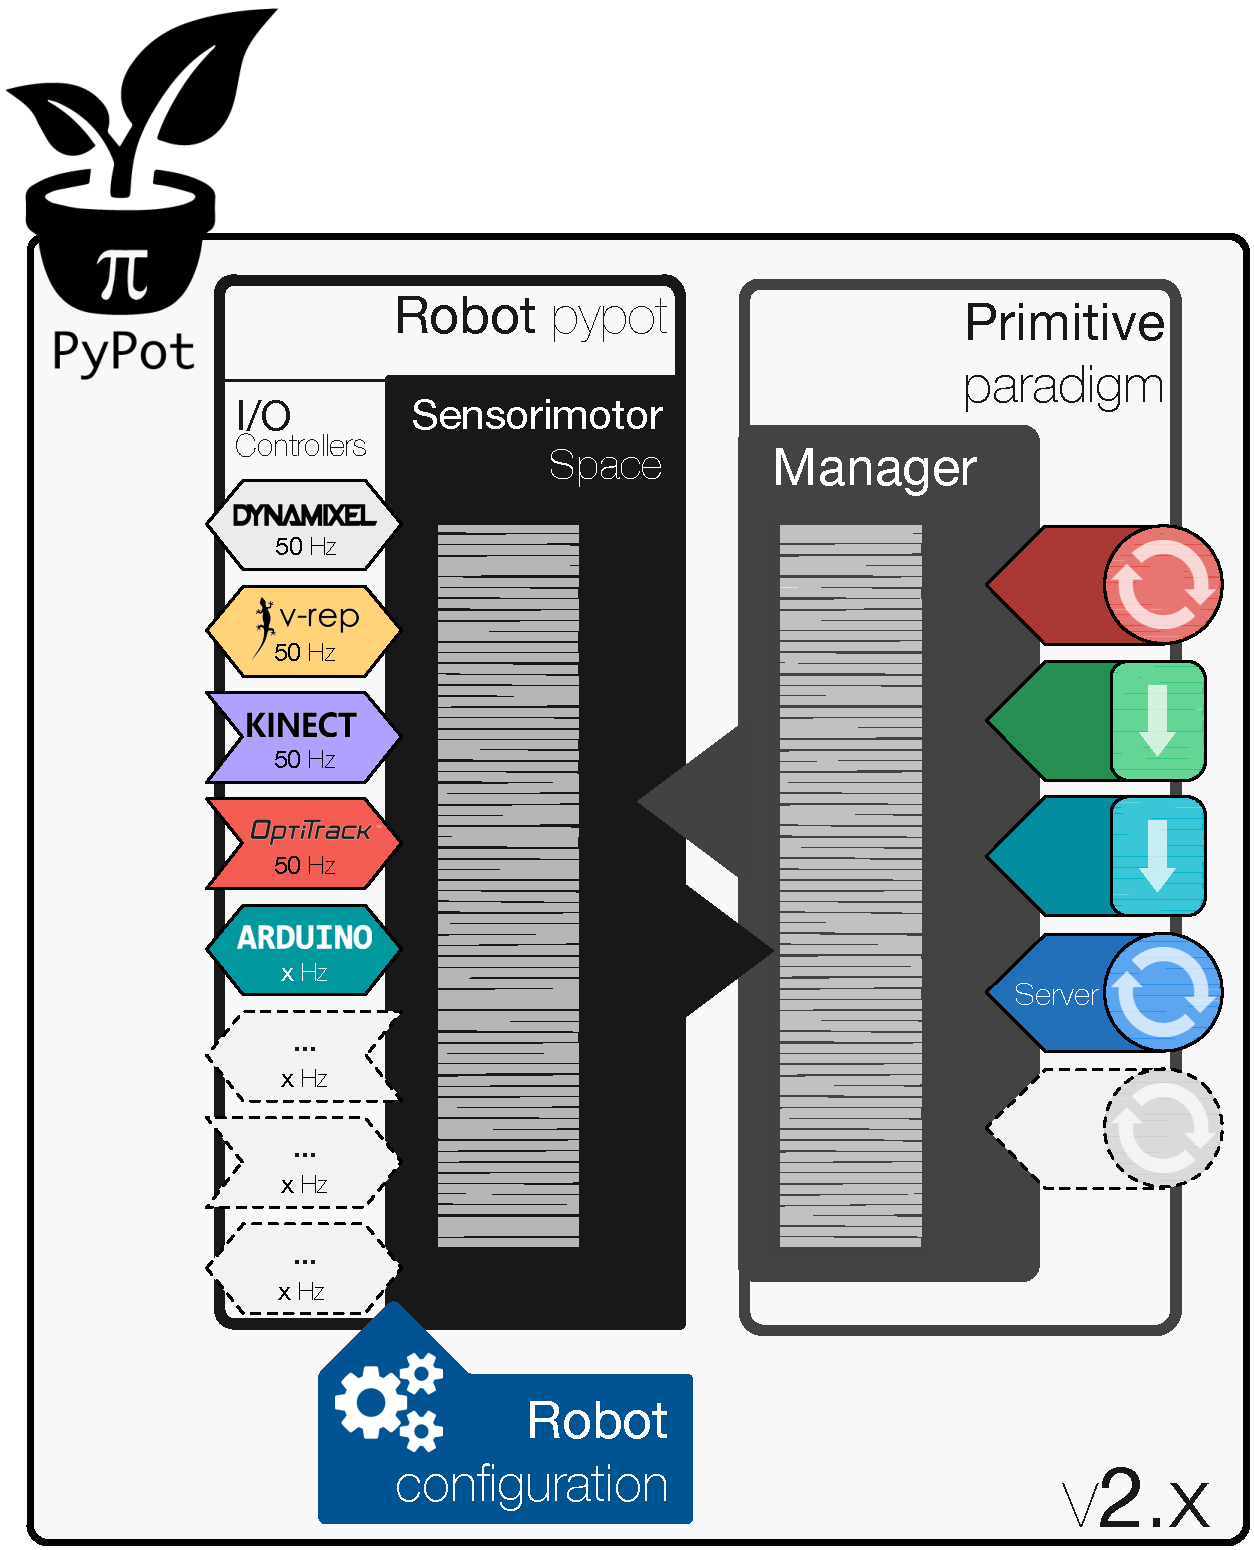
\includegraphics[width=\linewidth]{pypot.pdf}
    \end{center}
    \caption{}
    \label{fig:pypot-modular-architecture}
\end{figure}


\subsection{I/O controllers} % (fold)
\label{sub:io-controllers}

The low-level Dynamixel controller presented previously (see section~\ref{sub:dynamixel-controller}) is actually an instance of an I/O controller. The I/O controllers are the interface between real world data acquisition and the pypot core. They constitute the low-level modular part of pypot and allow for anyone to create a custom controller adapted to particular robot properties.

A brilliant example of this modular I/O controller architecture is the control of the robot either in the simulator or the real world just by switching between I/O controllers:

\subsubsection{Switching between the simulator and the real world} % (fold)

As it is often easier to work in simulation rather than with the real robot, Pypot has been linked with the V-REP simulator\footnote{\url{http://www.coppeliarobotics.com/features.html}}. It is described as the “Swiss army knife among robot simulators” and is indeed a very powerful tool to quickly (re)create robotics setup. Moreover, we chose to integrate this particular simulator first because it shares distinctive features with the Poppy project, i.e. being cross-platform, easy-to-use, extensible and open source\footnote{Actually V-REP has a double license Commercial/GPL so either one pays and can keep his customizations or has to release all modification under GPL.}

\begin{figure}[tb]
    \begin{center}
        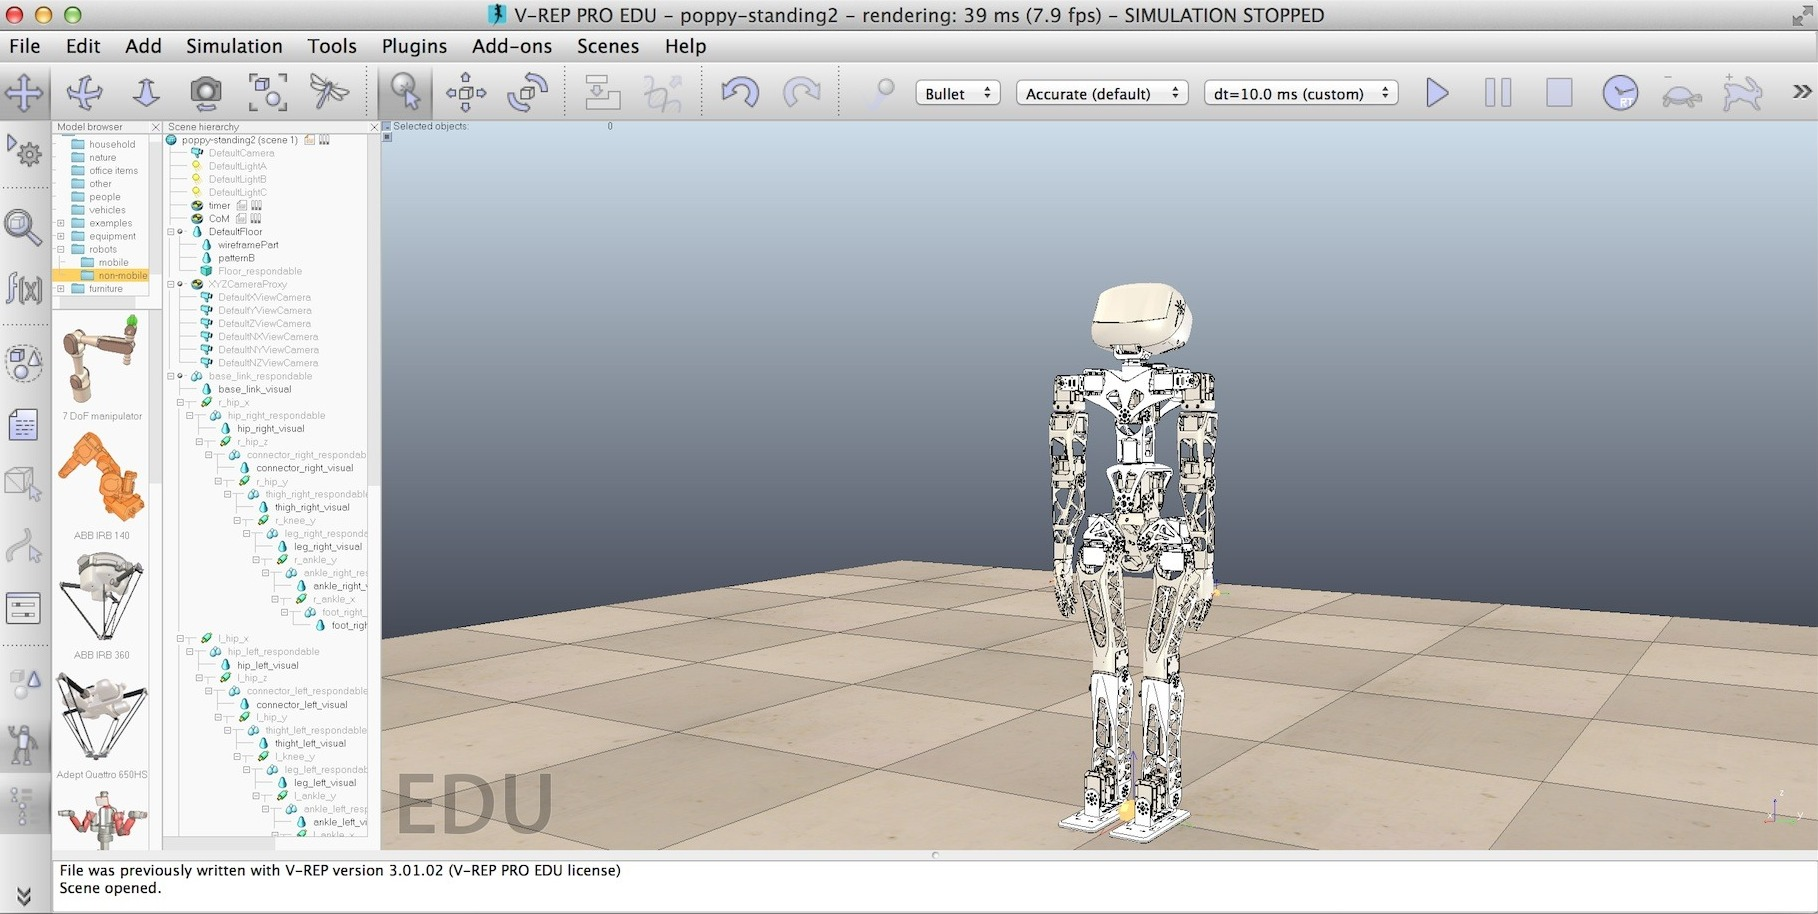
\includegraphics[width=\linewidth]{pypot_vrep.jpg}
    \end{center}
    \caption{}
    \label{fig:pypot-vrep}
\end{figure}


The connection with V-REP was created using the I/O controllers presented previously and the V-REP’s remote API.
Thanks to the low-level modularity of pypot, it permits to seamlessly switch from your real robot to the simulated one because it only requires switching the low-level I/O controller from the Dynamixel (\emph{DxlController} class) one to the V-REP one (\emph{VrepController} class).

The switch between the simulation and the real robot is possible with a single line of code, and in most case, only requires changing the way the robot is instantiated see \codename~\ref{code:vrep_pypot_switch}.

\lstinputlisting[
    language = Python,
    caption = {},
    label = {code:vrep_pypot_switch},
    float = ht]
    {code/vrep_pypot_switch.py}

In addition, it provides some extended features relative to the needs we have in a robot simulator, among them:
load a scene, start/stop/restart a simulation, pause/resume the simulation, get an object position/orientation.
Yet not all Dynamixel registers have their V-REP equivalent. For the moment, only the control of the position is used but it will be extended in the future. Also more advanced features can be easily added thanks to the controller abstraction.


\subsubsection{Custom I/O controllers} % (fold)

The I/O controller is actually defined by two classes:

\begin{itemize}
    \item the IO class defining how to communicate with an object (i.e. motor or sensor) and obtain its data,
    \item the controller class defining all object properties the robot can access and control.
\end{itemize}

It is therefore possible to extend the number of controllers to any connected object. For example, it could be used to change the type of motors used and replace the Robotis motors with more low-cost ones, or to control a robot with a simulator other than V-REP, and the switch should be as straightforward.


\textbf{TODO put code ?}


\subsubsection{Automatic generation of the robot} % (fold)
In the same way that the pypot robot class can automatically create a robot based on Dynamixel motors and generate an easy-to-use API, it can handle the variability of the I/O controllers. Indeed the desired I/O controllers can be indicated during the robot configuration then the robot will be generated in accordance with the specified controllers. The v-rep simulator is an example of such use (\codename~\ref{code:vrep_pypot_switch}).

Thus the pypot robot can handle multiple controllers both for motor control and for the sensors acquisition (e.g. IMU, tactile, camera).


\subsection{Primitive paradigms} % (fold)
\label{sub:primitive-paradigms}

The high-level modularity of pypot is expressed by the primitive paradigms. We call a Primitive any simple or complex behaviour applied to a Robot. A primitive can access all sensors and effectors in the robot. A primitive is supposed to be independent\footnote{The independence of primitives is really important when one creates complex behaviours - such as balance - where many primitives are needed. Adding another primitive - such as walking - should be direct and not force the rewriting of everything. Furthermore, the balance primitive could also be combined with another behaviour - such as shooting a ball - without modifying it.} from other primitives. In particular, a primitive is not aware of the other primitives running on the robot at the same time. We imagine those primitives as elementary blocks that can be combined to create more complex blocks in a hierarchical manner.

To ensure this independence, the primitive is running in a sort of sandbox. More precisely, this means that the primitive does not have direct access to the robot. It can only request commands (e.g. set a new goal position of a motor) to a Primitive Manager, which transmits them to the “real” robot. As multiple primitives can run on the robot at the same time, their request orders are combined by the manager\footnote{The primitives all share the same manager. In further versions, we would like to move from this linear combination of all primitives toward a hierarchical structure and have different layer of managers.}.

The manager uses a filter function to combine all orders sent by primitives. By default, this filter function is a simple mean but you can choose your own specific filter (e.g. add function).

To write a primitive, the user only needs to create a subclass of the Primitive class. It provides basic mechanisms (e.g. connection to the manager, setup of the thread) to allow the direct “plug” of novel primitives to a robot and run it.

Currently there are two kinds of primitives.


\lstinputlisting[
    language = Python,
    caption = {},
    label = {code:primitive},
    float,
    floatplacement = h]
    {code/primitive.py}

\lstinputlisting[
    language = Python,
    caption = {},
    label = {code:loop_primitive},
    float,
    floatplacement = h]
    {code/loop_primitive.py}

The primitive can be start(), stop(), pause() and resume(). Unlike a regular python thread, a primitive can be restarted by calling the start() method again.

When overriding the Primitive, you are responsible for correctly handling those events. For instance, the stop method will only trigger the \emph{should\_stop} event that you should watch in your run loop and break when the event is set. In particular, you should check the should\_stop() and should\_pause() in your run loop. You can also use the wait\_to\_stop() and wait\_to\_resume() to wait until the commands have actually been executed.


\lstinputlisting[
    language = Python,
    caption = {},
    label = {code:start_primitive},
    float,
    floatplacement = h]
    {code/start_primitive.py}

\lstinputlisting[
    language = Python,
    caption = {},
    label = {code:attach_primitive},
    float,
    floatplacement = h]
    {code/attach_primitive.py}

The move feature described in section~\ref{sub:move_recording} is actually based on the pypot primitive paradigm. More precisely, the \emph{MoveRecorder} and \emph{MovePlayer} are defined as a subclass of \emph{LoopPrimitive}.

\subsection{Extensible API} % (fold)

We added the possibility to remotely access and control your robot through the TCP network. This can be useful both to work with client/server architecture (e.g. to separate the low-level control running on an embedded computer and higher-level computation on a more powerful computer) and to allow you to plug your existing code, written in another language, into the pypot’s API.

We defined a protocol that allows all the robot variables and methods (including motors and primitives) to be accessed via a JSON request. The protocol is entirely described in the section Protocol below. Two transport methods have been developed so far:

\subsubsection{HTTP server} % (fold)

The \emph{HTTPServer }is based on the bottle python framework (http://bottlepy.org/). We have developed a sort of REST API based on the protocol described above:

\begin{itemize}
    \item GET /motor/list.json
    \item GET /primitive/list.json
    \item GET /motor/<name>/register.json (or GET /<name>/register.json)
    \item GET /motor/<name>/<register> (or GET /<name>/<register>)
    \item POST /motor/<name>/<register> (or POST /<name>/<register>)
    \item POST /primitive/<prim\_name>/call/<meth\_name> (or GET /<prim\_name>/call/<meth\_name>)
    \item POST /request.json
\end{itemize}


\lstinputlisting[
    language = Python,
    caption = {},
    label = {code:http_server},
    float,
    floatplacement = h]
    {code/http_server.py}


\subsubsection{ZMQ server} % (fold)

The Zmq Server used a Zmq socket to send (resp. receive) JSON request (JSON answer). It is based on the REQ/REP pattern. So you should always alternate sending and receiving. It will probably be switched to PUB/SUB soon.

Zmq has been chosen as it has been bound to most languages\footnote{\url{http://zeromq.org/bindings:_start}} and can thus be used to connect code in other languages to pypot. For instance, we used it to connect RLPark\footnote{RLPark is a Java reinforcement learning library developed by Thomas Degris to experiment with online learning algorithms on robots and benchmarks, see \url{http://rlpark.github.io/}} to pypot.

The Zmq server is faster than the HTTP version and should be preferred when working with high frequency control loops.

\lstinputlisting[
    language = Python,
    caption = {},
    label = {code:zmq_server},
    float,
    floatplacement = h]
    {code/zmq_server.py}


In particular, those for which the extension could be used to create a monitor interface using web technology.



\section{Discussion} % (fold)

\subsection{Why not using ROS instead ?} % (fold)

One famous robotics software is the Robot Operating System\footnote{The Robot Operating System (ROS) is a flexible framework for writing robot software. It is a collection of tools, libraries, and conventions that aim to simplify the task of creating complex and robust robot behaviour across a wide variety of robotic platforms.}. ROS is very widespread in the research community and one could quite rightly question the choice we made in creating a whole new architecture rather than using a well-known and efficient one.

Actually ROS has several aspects that do not fit in with the objectives we have. Indeed, using ROS is not a simple task. The installation is only recommended on one precise Ubuntu distribution\footnote{ROS Hydro only supports Precise, Quantal, and Raring for debian packages \url{http://wiki.ros.org/indigo/Installation}}, and the whole architecture is of course powerful but difficult to set and maintain. Also changing the low-level is complex and requires hacks, sometimes not very elegant ones. Finally, ROS require high computational power, which make it difficult to embed on small computers.

In the Poppy project, we are trying to create a multidisciplinary robotic community, involving as a result, non-robotics experts. Thus, we endeavour to bring down the complexity of using Poppy. To reach this goal, we need a simple user interface/API and a lightweight library, easy to setup whichever system used. Finally, ROS is very modular for high-level but we desire to have modular low-level control.

For all the reasons mentioned above, we considered it to be more simple and effective to create a novel lightweight robot control library rather than adapting ROS to our needs.


\subsection{Limitations} % (fold)

The pypot library is currently rather mature and robust, yet there remain some limitations that are challenging to a variable degree.

\subsubsection{Performances}

Pypot is written in python because it allows fast development and simple API for non-expert users. Also the main goal of pypot is to be an easy-to-use prototyping environment so users can run complete experiments with a custom robot in a couple of minutes to few hours. These choices imply a number of layers and multiple calls of functions, slowing the general execution of the code.

While it is not a problem on modern personal computers, it is more limiting on very light configurations (see \figurename~\ref{fig:pypot-board-comparaison}). For example, running pypot on a Raspberry Pi takes all CPU resources and the sensorimotor acquisition of Poppy at $50Hz$ (i.e. $<20ms$) is not achieved.
The performance could be improved by splitting pypot with the low-level executed on

\begin{figure}[tb]
    \begin{center}
        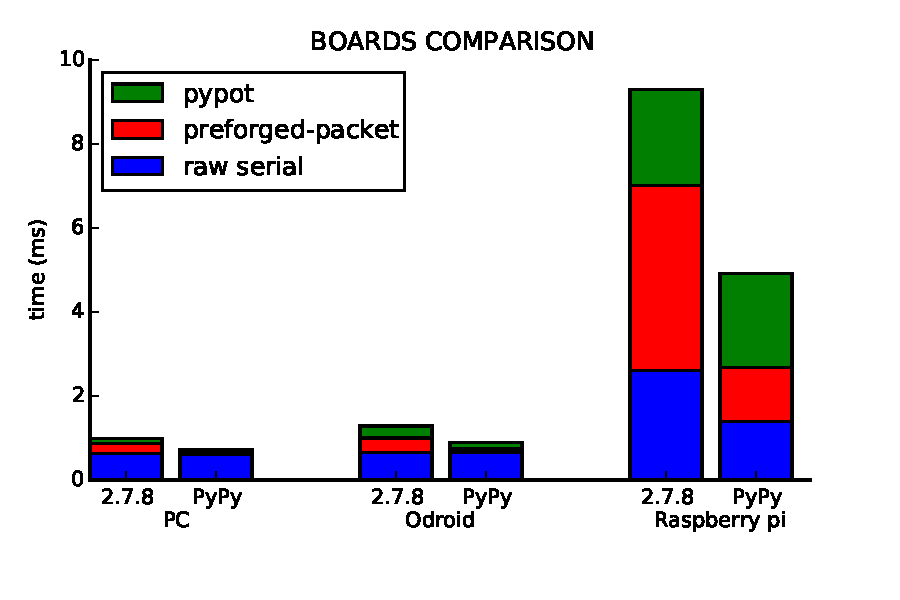
\includegraphics[width=0.7\linewidth]{board-cmp.pdf}
    \end{center}
    \caption{Time spent to communicate with one motor.}
    \label{fig:pypot-board-comparaison}
\end{figure}

\begin{figure}[tb]
\centering
    \subfloat[][ CPU load during pypot run]{\label{fig:cpu-load}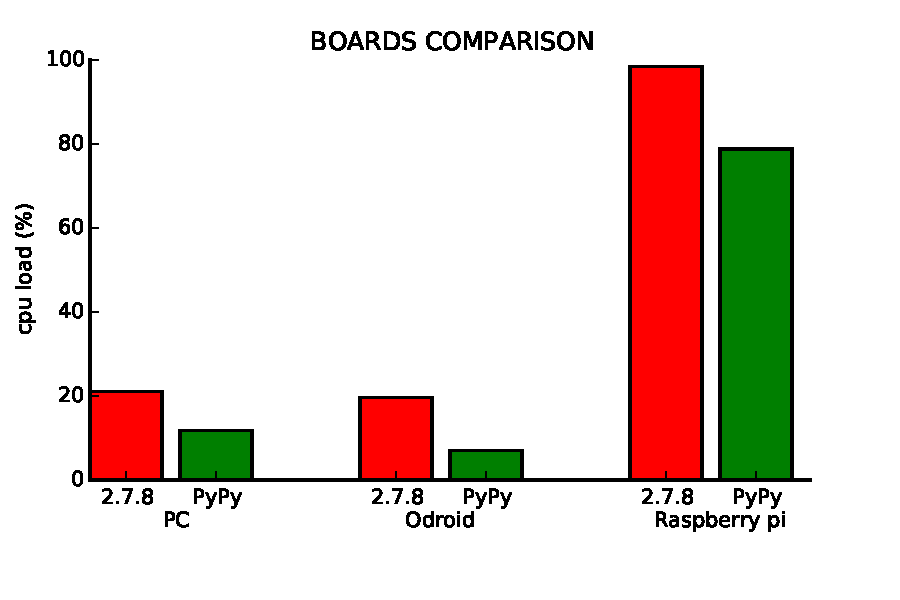
\includegraphics[width=0.5\linewidth]{cpu_load.pdf}}
    \hfil
    \subfloat[][Time spend to synchronize the 25 Poppy's motors]{\label{fig:pypy-opti}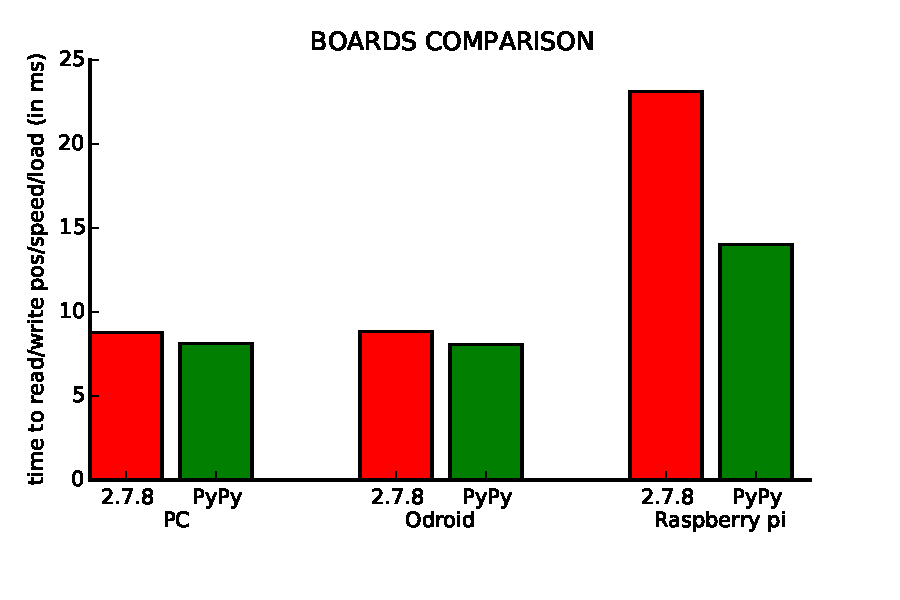
\includegraphics[width=0.5\linewidth]{controller.pdf}}
    \caption{}
    \label{fig:pypot-run}
\end{figure}



\subsubsection{The primitive paradigms: The Good, the Bad and the Ugly}

The use of primitives (see section~\ref{sub:primitive-paradigms}) raises some complicated limitations. Indeed it is really convenient to run complex behaviours by splitting them into more simple ones but the interaction between primitives is really complex to manage and can lead to undesired behaviours. Indeed, while multiple primitives can request to change the same value, the final value is the result of the combination (e.g. mean, sum) of several primitives.


It is a case of emergent behaviour\footnote{Finding the rules that can lead to a desired behaviour is more difficult than explaining the real, observable complex behaviour of an agent interacting with its environment. Since the behaviour itself cannot be preprogramed but is always the result of an agent-environment interaction, we must design for emergence rather than directly for a specific behaviour~\parencite{Pfeifer06}.} problem as explained in chapter~\ref{cha:morphology-review}, but at the control software level. It is really interesting because it forces us to design  for emergence as explained by Steels~\parencite{Steels1991emergence}, yet it is still challenging to explain to the end user and in particular to non-expert ones.


\section{Conclusion} % (fold)

As explained in this chapter, Pypot is a modular robot control library, simple to use and extendable to the needs of users. Moreover its very modular low-level permits to easily manage morphological variability while its high-level primitive paradigm permits to quickly run more or less complex behaviour on the robot.

Pypot is open source and distributed under GPLv3 license. All sources are available on the GitHub repository of the project: \url{https://github.com/poppy-project/pypot}. Also the complete documentation can be accessed here: \url{https://poppy-project.github.io/pypot/}.


% subsection _ (end)

% The high-level design allows the use of primitives.
% Primitives are ...
% This features is really powerful as it allows the creation of complex behaviour as a sum of simple behaviour.
% However, the interaction between them is tricky and can lead to undesired behaviour.


% \lstinputlisting[
%     language = Python,
%     caption = {},
%     label = {code:mockup_motor},
%     float,
%     floatplacement = h]
%     {code/mockup.py}



